\documentclass[a4paper,12pt]{report}
\usepackage{graphicx} 		% images
\usepackage[utf8]{inputenc}	% encoding: UTF-8
\usepackage[italian]{babel}	% language
\usepackage[margin=0.5in, includefoot]{geometry}	% margin
\usepackage{scrextend}		% KOMA scripts?
\usepackage{array}			% table width
\usepackage[table]{xcolor}	% table colors
\usepackage{tocloft}			% table of contents
\usepackage{hyperref}			% hyperlinks inside document
\usepackage[italian]{cleveref}	% ^
\usepackage[section]{placeins}
\usepackage{float}
\usepackage{listings}
\usepackage{color}

\renewcommand{\cftsecleader}{\cftdotfill{\cftdotsep}}
% this command makes a chapter without number and adds it to the toc
\newcommand\chap[1]{
    \chapter*{#1}
    \addcontentsline{toc}{chapter}{#1}
    \markboth{#1}{#1}}

% same as above, but for sections
\newcommand\sect[1]{
    \section*{#1}
    \addcontentsline{toc}{section}{#1}
    \markboth{#1}{#1}}

% colors used in tables and code listings
\definecolor{keywordcolor}{HTML}{2e5abd}
\definecolor{morekwcolor}{HTML}{ff1a8d}
\definecolor{strcolor}{rgb}{0.58,0,0.82}
\definecolor{tablinecolor}{HTML}{999da1}
\definecolor{rowc}{HTML}{abc3f5}

\newcolumntype{P}[1]{>{\centering\arraybackslash}p{#1}}
\renewcommand{\arraystretch}{1.8}
\arrayrulecolor{tablinecolor} % table lines color

\renewcommand\lstlistingname{Quelltext} % change language of section name
% general setup for listings
\lstset{
    language=SQL,
    basicstyle=\ttfamily\footnotesize,
	breakatwhitespace=false,
	breaklines=true,
    tabsize=4,
    columns=fixed,
    showstringspaces=false,
    commentstyle=\color{keywordcolor},
    keywordstyle=\color{blue},
    numberstyle=\color{strcolor},
    stringstyle=\color{strcolor},
    classoffset=3,
    morekeywords={now, datediff},
    keywordstyle=\color{morekwcolor}
}

\title{
\Huge \textbf{Elaborato per il corso di Basi di Dati} \\
[4mm]
\large A.A. 2020/2021 \\
\large Progetto di una base di dati per la gestione di un servizio online
}
\author{Christian Ricci \\
christian.ricci3@studio.unibo.it \\
0000915693}



%%%%%%%%%%%%%%%%%%%%%%%%%%%%%%%%%
% Document begin
%%%%%%%%%%%%%%%%%%%%%%%%%%%%%%%%%



\begin{document}

\maketitle
\tableofcontents

\chap{Analisi dei requisiti}

Si vuole realizzare un database per gestire un servizio online di videogiochi. Il database dovrà immagazzinare dati relativi ai videogiochi, agli utenti, alle iscrizioni. Gli utenti potranno {giocare} accedendo al servizio e potranno partecipare in sessioni multiplayer. I direttori del servizio potranno aggiungere nuovi videogiochi, consultare statistiche riguardanti gli utenti, etc.

\sect{Definizione delle specifiche in linguaggio naturale}

Il testo ottenuto dall'intervista con l'azienda è il seguente:\\\\

\begin{addmargin}[4em]{4em}
La casa produttrice di videogiochi GameSoft vuole realizzare un servizio online per tutti i videogiochi che ha pubblicato in passato. Gli utenti che si registreranno a questo nuovo servizio potranno accedere ad un catalogo di videogiochi e potranno giocare liberamente a qualunque gioco nel catalogo senza ulteriori costi. Degli utenti si vuole tener traccia del nome utente, della password, dell'email, dell'età e anche di un numero di telefono. Il numero di telefono è opzionale e un utente lo può dare anche dopo essersi registrato.

Al momento della registrazione l'utente potrà scegliere tra tre piani: il primo prevede un periodo gratuito di un mese, che non si potrà rinnovare; a quel punto l'utente deve decidere tra gli altri due piani. Il secondo piano prevede un costo e comporta l'iscrizione al servizio per un mese. Il terzo piano, invece, comporta l'iscrizione per un anno. Si vuole anche memorizzare lo storico delle iscrizioni per ogni utente.

Per ogni videogioco si vuole memorizzare il titolo, il genere, l'anno di rilascio, l'azienda sviluppatrice e il produttore esecutivo. Per ogni utente del servizio si vuole anche dare la possibilità di acquistare una copia fisica di qualunque videogioco, che, però, potrebbe anche non essere disponibile. Ogni videogioco può avere più copie fisiche, ma il prezzo di ogni copia del videogioco è la stessa. Si vuole anche memorizzare lo storico degli acquisti per ogni utente.

Ogni utente inoltre dovrebbe essere in grado di visualizzare il profilo di altri utenti, e di sapere alcune statistiche su quell'utente: le ore di gioco, sia giornaliere che totali; una lista dei giochi più giocati dall'utente; una lista dei giochi preferiti dall'utente. Altre statistiche appaiono per i videogiochi: una lista dei videogiochi più giocati da ogni utente e una lista dei giochi più amati.

Infine, si vuole anche immagazzinare anche alcune informazioni relative al multiplayer. Gli utenti del servizio possono iniziare una sessione di gioco con altri utenti e scegliere un videogioco da giocare: si vuole memorizzare i dati di ogni sessione, che includeranno gli utenti partecipanti, il videogioco scelto e il tempo trascorso a giocare in multiplayer. Si vuole anche mantenere uno storico delle sessioni per ogni utente. Ovviamente, si dovrebbe tener conto che il gioco scelto sia effettivamente un gioco multiplayer. \\\\

\end{addmargin}

\sect{Estrazione dei concetti fondamentali}

I concetti principali sono riassunti in questa tabella.

\begin{table}[h!]
\begin{center}
	\begin{tabular}{ | m{4cm} m{8cm} m{5cm} | }
	\rowcolor{rowc}
	\textbf{Termine} & \textbf{Breve descrizione} & \textbf{Eventuali sinonimi} \\
	Utente & Colui che accede al servizio. Può sottoscrivere nuovi piani, iniziare nuove partite con i videogiochi presenti, creare o partecipare a sezioni, comprare copie fisiche di un gioco. & Account, Profilo utente, Profilo giocatore \\ \hline
	Videogioco & Indica un videogioco del catalogo. & Titolo \\ \hline
	Copia & Indica una copia fisica di un videogioco. Ogni videogioco può avere più copie fisiche. & Copia videogioco, Copia fisica \\ \hline
	Piano & Ogni utente deve sottoscrivere un piano per accedere al servizio. & Abbonamento, Iscrizione\\ \hline
	Sessione di gioco & Una partita di un videogioco multiplayer, creata inizialmente da un utente. & Sessione \\ \hline
	\end{tabular}
\end{center}
\caption{La tabella dei concetti principali.}
\end{table}

A seguito della lettura e comprensione dei requisiti richiesti dal cliente, si procede sviluppando un testo che
ne riassuma tutti i concetti e in particolare ne estragga quelli principali, risultando essere in questo modo
meglio fruibile per la realizzazione della base di dati.\\\\

\begin{addmargin}[4em]{4em}
Per ogni \textbf{\textit{utente}} si memorizza nome, cognome, password, email, età e opzionalmente numero di telefono. Ogni utente deve avere un codice univoco, fornito al momento della registrazione.

Un utente può sottoscrivere più \textbf{\textit{piani}}: un piano gratuito è attivato al momento della registrazione. Per ogni tipo di piano c'è una durata e un prezzo e ogni piano viene mantenuto in uno storico, in cui si memorizza anche la data d'inizio (non c'è bisogno della data di scadenza, dato che si può evincere dal tipo di piano). Ogni utente può avere un solo piano attivo alla volta.

Per ogni \textbf{\textit{videogioco}} si deve memorizzare titolo, genere, anno di rilascio, azienda sviluppatrice e produttore esecutivo. Si devono anche memorizzare prezzo e quantità di copie per ogni videogioco. Per ogni copia, invece, si deve memorizzare la data di acquisto.

Infine, per ogni \textbf{\textit{sessione}} occorre memorizzare gli utenti partecipanti e il gioco scelto. Dato che non tutti i giochi permettono di giocare in multiplayer, bisogna fare una distinzione tra \textbf{\textit{gioco single player}} e \textbf{\textit{gioco multiplayer}}. Si suppone, inoltre, che un videogioco multiplayer abbia un numero minimo e massimo di giocatori. \\\\

\end{addmargin}

Da questo testo si può anche evincere le principali azioni richieste:

\begin{enumerate}
\item Login di un utente
\item Registrare la sottoscrizione di un piano
\item Registrare la cancellazione di un piano
\item Cercare un gioco per titolo/genere/azienda e usando un filtro
\item Visualizzare i giochi più giocati e quelli più preferiti
\item Registrare l'acquisto di una copia di un videogioco
\item Cercare un utente usando un filtro
\item Visualizzare il numero di ore di gioco giornaliero e totale di un utente
\item Visualizzare i giochi preferiti di un utente
\item Aggiungere un gioco tra i preferiti
\item Registrare la creazione di una sessione di gioco
\item Visualizzare quante sessioni un utente ha creato o ha partecipato per un videogioco
\item Visualizzare il profitto mensile del servizio
\end{enumerate}


%%%%%%%%%%%%%%%%%%%%%%%%%%%%%%%%%%%%%%%%%%%%
% schema concettuale
%%%%%%%%%%%%%%%%%%%%%%%%%%%%%%%%%%%%%%%%%%%%


\chap{Progetto dello schema concettuale}

La strategia adottata per creare lo schema concettuale è una strategia mista, orientata al bottom-up. Il database è composto da più ambiti, che verranno analizzati e raffinati uno ad uno, per poi creare uno schema finale che comprenda tutto il database.

\sect{Schema scheletro}

L'associazione tra \textbf{Utente} e \textbf{Piano} è abbastanza evidente: un utente può sottoscrivere più piani, ed ogni piano può avere una diversa tipologia. Inoltre, un piano può essere cancellato in qualunque momento dall'utente: per rappresentare questa relazione, si è pensato di creare una gerarchia di tipo \textit{Subset}: \textbf{Piano Cancellato} specializza Piano. L'entità Piano servirà inoltre per rappresentare lo storico dei piani, dato che l'intervista non ha posto particolari requisiti sullo storico. Ogni piano memorizza anche la data e l'ora di acquisto: avere anche l'ora preverrà il problema che un utente non riesca a sottoscrivere un nuovo piano nello stesso giorno (si pensi al caso in cui un utente sottoscriva un piano, poi lo cancelli e ne sottoscriva un altro nello stesso giorno).

L'entità Piano non memorizza alcuna data finale. Per capire il vero stato del piano (in corso, finito o cancellato) e la fine, occorrerà guardare anche la sua tipologia. Dato che ci sono tre diverse tipologie, ognuna con diverse proprietà, si è pensato di reificare la tipologia nell'entità \textbf{Tipologia piano}. Per rappresentare i tre tipi di piano, si è scelto di usare specializzazioni per la più generica Tipologia piano. Riguardo agli identificatori, sia Utente che Piano hanno identificatori univoci, mentre la tipologia piano sarà identificata dal piano in sé.

Un'utente non può stipulare un piano se ha già un piano in corso: questo vincolo non si può esprimere con facilità nello schema concettuale, perciò sarà inserito come \textit{business rule}.

\begin{figure}[!htb]
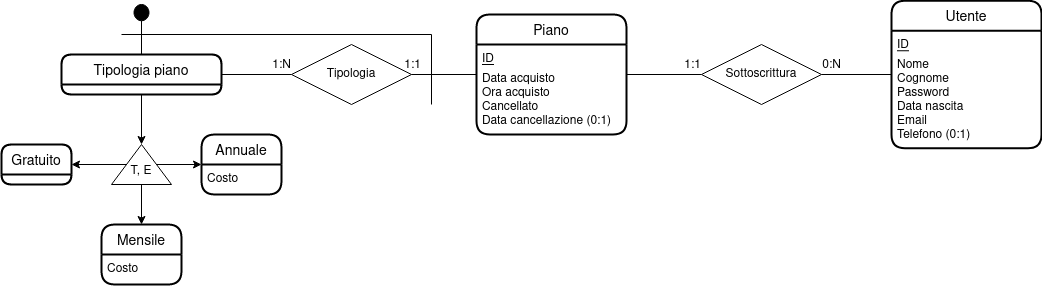
\includegraphics[width=\textwidth]{piano.png}
\caption{Lo schema Entity-Relationship relativo at utenti e piani.}
\label{img:schema_piano}
\end{figure}

Riguardo alle relazioni tra Utente e Videogioco, abbiamo una relazione che riguarda le statistiche dell'utente ed una che riguarda l'acquisto di copie fisiche di un videogioco da parte degli utenti.

Le statistiche di cui si vuole tener traccia sono principalmente due: le ore di gioco dell'utente e i giochi preferiti dell'utente. Per le ore di gioco, si è deciso di rappresentarle tramite un'entità partita: ogni partita di un utente deve essere comunque tracciata per sapere le ore di gioco, quindi ogni partita è rappresentata dall'ID dell'utente, dall'ID del videogioco e dalla data e l'ora di quando è stata iniziata.

Per i giochi preferiti dell'utente, basta avere un'associazione tra Utente e Videogioco che indica la preferenza di un utente per quel videogioco. Mediante operazioni a lato software si potranno estrapolare le altre statistiche richieste, ad esempio la lista dei giochi preferiti e la lista dei giochi più giocati.

Dato che per un videogioco ci possono essere più copie fisiche, si è scelto di creare un entità anche per Copia Videogioco. Il prezzo di ogni copia non riguarda le singole copie, bensì riguarda il gioco in sé, e si suppone inoltre che questo dato rimanga costante nel tempo, per cui è stato messo come attributo di videogioco. Una copia può anche rimanere invenduta, quindi si è pensato di immagazzinare il dato relativo alla data di acquisto come attributo dell'associazione Acquisto. Ogni copia è identificata tramite un codice univoco e l'associazione al videogioco di cui è copia.

\begin{figure}[!htb]
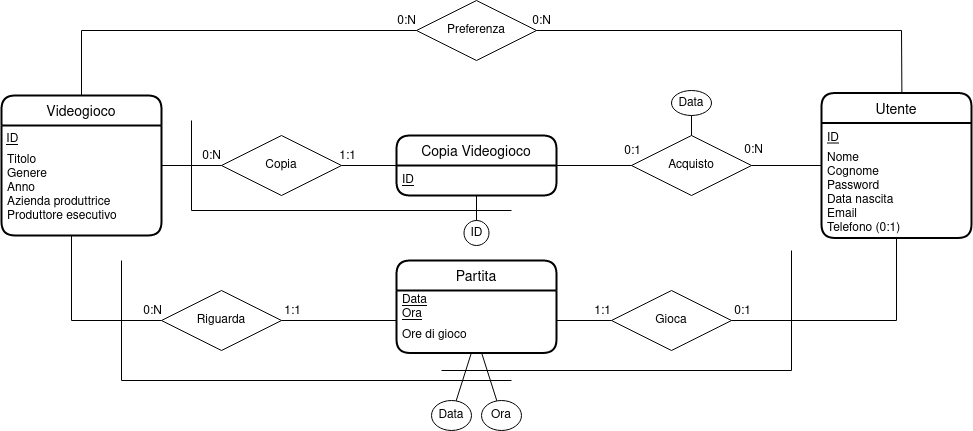
\includegraphics[width=\textwidth]{vg.png}
\caption{Lo schema Entity-Relationship relativo agli utenti, videogiochi, copie e statistiche.}
\label{img:schema_vg}
\end{figure}

L'ambito relativo alle sessioni di gioco multiplayer è il più semplice.

Un \textbf{Videogioco multiplayer} è una specializzazione di Videogioco ed aggiunge gli attributi di numero minimo e massimo di giocatori. Le due entità Utente e Videogioco Multiplayer sono associate all'entità \textbf{Sessione}, che raccoglie dati relativi alla specifica sessione. Una sessione è identificata dall'attributo ID di Sessione e dall'associazione con Videogioco Multiplayer.

Per sottolineare il fatto che un solo utente può dare inizio ad una sessione, mentre più utenti possono parteciparvi, si è optato per due associazioni, \textbf{Creazione} e \textbf{Partecipazione}, tra Utente e Sessione. Rimane un vincolo inespresso: in una sessione, il numero minimo e massimo di giocatori dipende dal videogioco, cosa difficile da esprimere usando il modello ER.

\begin{figure}[H]
\centering{}
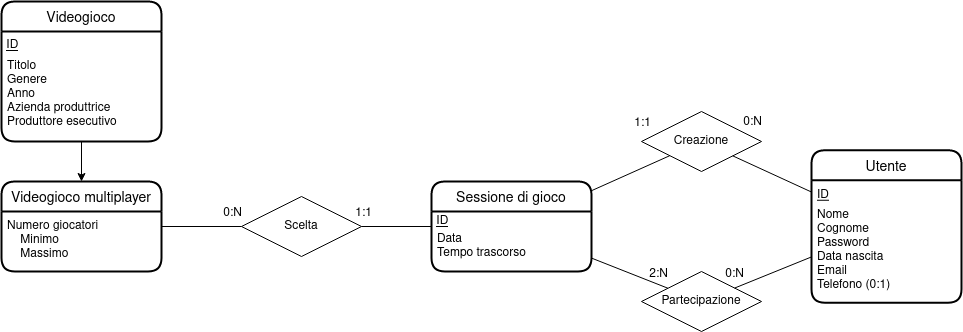
\includegraphics[width=\textwidth]{session.png}
\caption{Lo schema Entity-Relationship relativo alle sessioni.}
\label{img:schema_sessione}
\end{figure}

\newpage

\sect{Schema finale}

\begin{figure}[!htb]
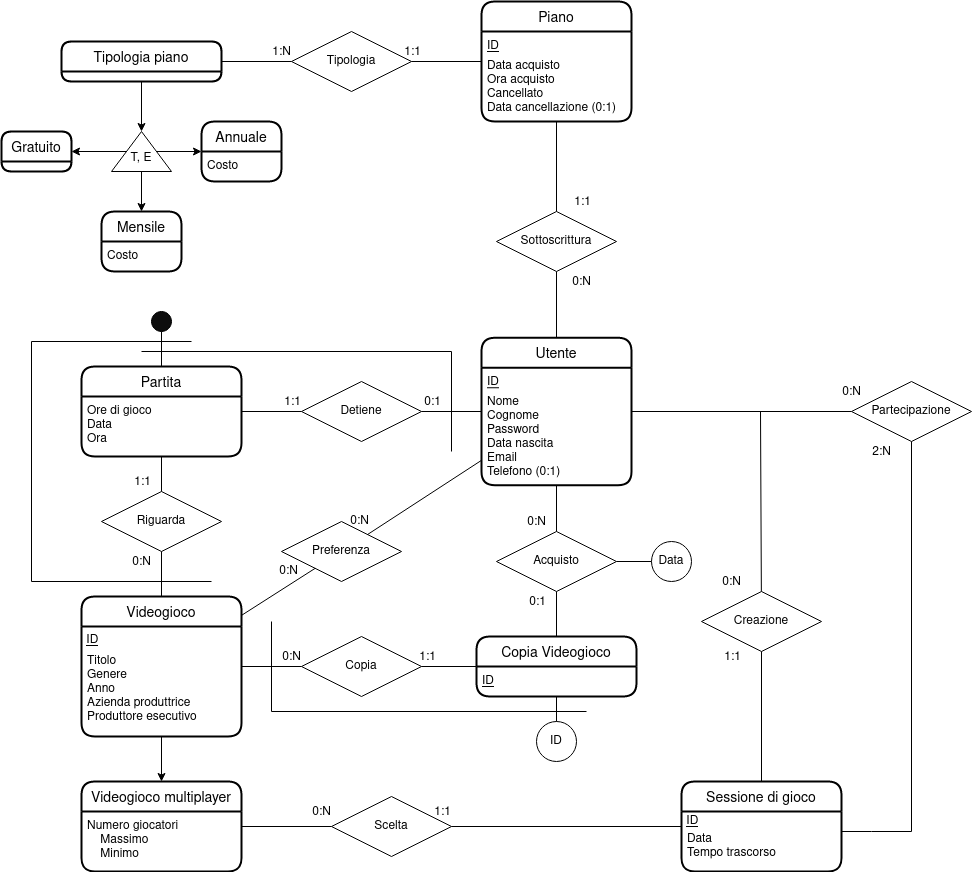
\includegraphics[width=\textwidth]{er_full.png}
\caption{Lo schema Entity-Relationship finale.}
\label{img:schema_finale}
\end{figure}

\newpage


%%%%%%%%%%%%%%%%%%%%%%%%%%%%%%%%%%%%%%%%%%%%
% progettazione logica
%%%%%%%%%%%%%%%%%%%%%%%%%%%%%%%%%%%%%%%%%%%%


\chap{Progettazione logica}

\sect{Stima del volume dei dati}

\begin{table}[h!]
\begin{center}
	\begin{tabular}{ | m{5cm} P{5cm} P{5cm} | }
	\rowcolor{rowc}
	\hline
    \textbf{Concetto} & \textbf{Costrutto} & \textbf{Volume} \\
	Utente & E & 10.000 \\ \hline
	Piano & E & 30.000 \\ \hline
	Sottoscrittura & R & 30.000 \\ \hline
	Tipologia piano & E & 3 \\ \hline
	Piano Cancellato & E & 3000 \\ \hline
	Videogioco & E & 1000 \\ \hline
	Copia Videogioco & E & 10.000 \\ \hline
	Copia & R & 10.000 \\ \hline
	Acquisto & R & 5000 \\ \hline
	Partita & E & 300.000 \\ \hline
	Gioca & R & 300.000 \\ \hline
	Riguarda & R & 300.000 \\ \hline
	Preferenza & R & 7000 \\ \hline
	Videogioco Multiplayer & E & 600 \\ \hline
	Sessione di gioco & E & 100.000 \\ \hline
	Scelta & R & 100.000 \\ \hline
	Creazione & R & 100.000 \\ \hline
	Partecipazione & R & 500.000 \\ \hline
	\end{tabular}
\end{center}
\caption{La tabella dei volumi.}
\end{table}

\sect{Descrizione delle operazioni principali e stima della loro frequenza}

Le operazioni principali sono elencate nella fase di analisi. Segue una tabella delle stime della frequenza per ogni operazione:

\begin{table}[h!]
\begin{center}
	\begin{tabular}{ | P{2cm} m{10cm} m{4cm} | }
	\rowcolor{rowc}
	\hline
	\textbf{Codice} & \textbf{Operazione} & \textbf{Frequenza} \\
	1  & Login di un utente & 1000 al giorno \\ \hline
    2  & Registrare la sottoscrizione di un piano & 200 al mese \\ \hline
    3  & Registrare la cancellazione di un piano & 50 al mese \\ \hline
    4  & Cercare un gioco per titolo/genere/azienda e usando un filtro & 3000 al giorno \\ \hline
    5  & Visualizzare i giochi più giocati e quelli più preferiti & 2000 al giorno \\ \hline
    6  & Registrare l'acquisto di una copia di un videogioco & 5 al giorno \\ \hline
    7  & Cercare un utente usando un filtro & 1000 al giorno \\ \hline
    8  & Visualizzare il numero di ore di gioco giornaliero e totale di un utente & 1000 al giorno \\ \hline
    9  & Visualizzare i giochi preferiti di un utente & 1000 al giorno \\ \hline
    10 & Aggiungere un gioco tra i preferiti & 5 al giorno \\ \hline
    11 & Registrare la creazione di una sessione di gioco & 100 al giorno \\ \hline
    12 & Visualizzare quante sessioni un utente ha creato o ha partecipato per un videogioco & 1000 al giorno \\ \hline
    13 & Visualizzare il profitto mensile del servizio & 1 al mese \\ \hline
	\end{tabular}
\end{center}
\caption{Tabella delle stime delle frequenze.}
\end{table}

\newpage

\sect{Schemi di navigazione e tabelle degli accessi}

In questa sezione sono riportate le tabelle degli accessi delle operazioni sopra descritte. Al fine del calcolo, si considerano gli accessi in scrittura di peso doppio rispetto a quelli in lettura.

\subsection*{1. Login di un utente}

\begin{table}[!htb]
\begin{center}
	\begin{tabular}{ | m{5cm} P{4cm} P{4cm} P{4cm} | }
	\rowcolor{rowc} \textbf{Concetto} & \textbf{Costrutto} & \textbf{Accessi} & \textbf{Tipo} \\
	Utente         & E & ? & L \\ \hline
	\rowcolor{rowc} \textbf{Totale}: & & & \\ \hline
	\end{tabular}
\end{center}
\end{table}

\subsection*{2. Registrare la sottoscrizione di un piano}

% per registrare la sottoscrizione, prima bisogna guardare se l'utente ha già un piano in corso.
Per permettere la registrazione di un nuovo piano, prima bisogna cercare se l'utente ha già un piano in corso: questo comporta anche accessi in lettura dei piani e delle tipologie.
In questa operazione, così come in molte altre, si suppone di avere già l'ID dell'utente che effettua l'operazione.

\begin{table}[!htb]
\begin{center}
	\begin{tabular}{ | m{5cm} P{4cm} P{4cm} P{4cm} | }
	\rowcolor{rowc} \textbf{Concetto} & \textbf{Costrutto} & \textbf{Accessi} & \textbf{Tipo} \\
	Sottoscrittura  & R & ? & L \\ \hline
	Piano           & E & ? & L \\ \hline
	Tipologia       & R & ? & L \\ \hline
	Tipologia piano & E & ? & L \\ \hline
	Sottoscrittura  & R & 1 & S \\ \hline
	Piano           & E & 1 & S \\ \hline
	\rowcolor{rowc} \textbf{Totale}: & & & \\ \hline
	\end{tabular}
\end{center}
\end{table}

\newpage

\subsection*{3. Registrare la cancellazione di un piano}

In maniera analoga all'ultima operazione, bisogna trovare il piano in corso dell'utente prima di poterlo cancellare.

\begin{table}[!htb]
\begin{center}
	\begin{tabular}{ | m{5cm} P{4cm} P{4cm} P{4cm} | }
	\rowcolor{rowc} \textbf{Concetto} & \textbf{Costrutto} & \textbf{Accessi} & \textbf{Tipo} \\
	Piano    		 & E & ? & L \\ \hline
	Tipologia		 & R & ? & L \\ \hline
	Tipologia piano  & E & ? & L \\ \hline
	Sottoscrittura   & R & ? & L \\ \hline
	Piano Cancellato & E & 1 & S \\ \hline
	\rowcolor{rowc} \textbf{Totale}: & & & \\ \hline
	\end{tabular}
\end{center}
\end{table}


\subsection*{4. Cercare un gioco per titolo/genere/azienda e usando un filtro}

\begin{table}[h!]
\begin{center}
	\begin{tabular}{ | m{4cm} P{4cm} P{4cm} P{4cm} | }
	\rowcolor{rowc} \textbf{Concetto} & \textbf{Costrutto} & \textbf{Accessi} & \textbf{Tipo} \\
	Videogioco       & E & ? & L \\ \hline
	\rowcolor{rowc} \textbf{Totale}: & & & \\ \hline
	\end{tabular}
\end{center}
\end{table}

\subsection*{5. Visualizzare i giochi più giocati e quelli più preferiti}

\begin{table}[h!]
\begin{center}
	\begin{tabular}{ | m{4cm} P{4cm} P{4cm} P{4cm} | }
	\rowcolor{rowc} \textbf{Concetto} & \textbf{Costrutto} & \textbf{Accessi} & \textbf{Tipo} \\
	Videogioco & E & ? & L \\ \hline
	Riguarda	   & R & ? & L \\ \hline
	Partita    & E & ? & L \\ \hline
	Preferenza & R & ? & L \\ \hline
	\rowcolor{rowc} \textbf{Totale}: & & & \\ \hline
	\end{tabular}
\end{center}
\end{table}

\newpage

\subsection*{6. Registrare l'acquisto di una copia di un videogioco}

Per registrare un acquisto, prima bisogna trovare se il videogioco in questione ha ancora copie disponibili: questo comporta anche l'accesso in lettura degli acquisti. Inoltre, per un eventuale sistema di pagamento, bisognerà anche cercare il prezzo del videogioco in questione (memorizzato per l'intero videogioco, non per ogni singola copia).

\begin{table}[h!]
\begin{center}
	\begin{tabular}{ | m{4cm} P{4cm} P{4cm} P{4cm} | }
	\rowcolor{rowc} \textbf{Concetto} & \textbf{Costrutto} & \textbf{Accessi} & \textbf{Tipo} \\
	Videogioco		 & E & ? & L \\ \hline
	Copia			 & R & ? & L \\ \hline	
	Copia Videogioco & E & ? & L \\ \hline
	Acquisto 		 & R & ? & L \\ \hline
	Acquisto 		 & R & 1 & S \\ \hline
	\rowcolor{rowc} \textbf{Totale}: & & & \\ \hline
	\end{tabular}
\end{center}
\end{table}

\subsection*{7. Cercare un utente usando un filtro}

\begin{table}[h!]
\begin{center}
	\begin{tabular}{ | m{4cm} P{4cm} P{4cm} P{4cm} | }
	\rowcolor{rowc} \textbf{Concetto} & \textbf{Costrutto} & \textbf{Accessi} & \textbf{Tipo} \\
	Utente & E & ? & L \\ \hline
	\rowcolor{rowc} \textbf{Totale}: & & & \\ \hline
	\end{tabular}
\end{center}
\end{table}

\newpage

\subsection*{8. Visualizzare il numero di ore di gioco giornaliero e totale di un utente}

\begin{table}[h!]
\begin{center}
	\begin{tabular}{ | m{4cm} P{4cm} P{4cm} P{4cm} | }
	\rowcolor{rowc} \textbf{Concetto} & \textbf{Costrutto} & \textbf{Accessi} & \textbf{Tipo} \\
	Utente  & E & ? & L \\ \hline
	Gioca   & R & ? & L \\ \hline
	Partita & E & ? & L \\ \hline
	\rowcolor{rowc} \textbf{Totale}: & & & \\ \hline
	\end{tabular}
\end{center}
\end{table}

\subsection*{9. Visualizzare i giochi preferiti di un utente}

\begin{table}[h!]
\begin{center}
	\begin{tabular}{ | m{4cm} P{4cm} P{4cm} P{4cm} | }
	\rowcolor{rowc} \textbf{Concetto} & \textbf{Costrutto} & \textbf{Accessi} & \textbf{Tipo} \\
	Preferenza & R & ? & L \\ \hline
	Videogioco & E & ? & L \\ \hline
	\rowcolor{rowc} \textbf{Totale}: & & & \\ \hline
	\end{tabular}
\end{center}
\end{table}

\subsection*{10. Aggiungere un gioco tra i preferiti}

% si suppone che il db prevenga coppie duplicate.

\begin{table}[h!]
\begin{center}
	\begin{tabular}{ | m{4cm} P{4cm} P{4cm} P{4cm} | }
	\rowcolor{rowc} \textbf{Concetto} & \textbf{Costrutto} & \textbf{Accessi} & \textbf{Tipo} \\
	Preferenza & R & 1 & S \\ \hline
	\rowcolor{rowc} \textbf{Totale}: & & & \\ \hline
	\end{tabular}
\end{center}
\end{table}

\newpage

\subsection*{11. Registrare la creazione di una sessione di gioco}

Si suppone di avere l'ID del videogioco scelto, l'ID dell'utente creatore e gli ID degli utenti partecipanti. Per registrare una sessione, bisogna cercare se il videogioco scelto è effettivamente un gioco giocabile in multiplayer (alternativamente, a lato software si possono filtrare i videogiochi non multiplayer) e che il videogioco supporti il numero di giocatori. Al momento della registrazione, si aggiornano opportunamente sia l'entità Sessione, sia le relazioni Creazione e Partecipazione.

\begin{table}[h!]
\begin{center}
	\begin{tabular}{ | m{4cm} P{4cm} P{4cm} P{4cm} | }
	\rowcolor{rowc} \textbf{Concetto} & \textbf{Costrutto} & \textbf{Accessi} & \textbf{Tipo} \\
	Videogioco multiplayer  	& E & ? & L \\ \hline
	Sessione					& E & 1 & S \\ \hline
	Scelta					& R & 1 & S \\ \hline
	Creazione				& R & 1 & S \\ \hline
	Partecipazione			& R & ? & S \\ \hline 
	\rowcolor{rowc} \textbf{Totale}: & & & \\ \hline
	\end{tabular}
\end{center}
\end{table}

\subsection*{12. Visualizzare quante sessioni un utente ha creato o ha partecipato per un videogioco}

\begin{table}[h!]
\begin{center}
	\begin{tabular}{ | m{4cm} P{4cm} P{4cm} P{4cm} | }
	\rowcolor{rowc} \textbf{Concetto} & \textbf{Costrutto} & \textbf{Accessi} & \textbf{Tipo} \\
	Partecipazione & R & ? & L \\ \hline
	Creazione      & R & ? & L \\ \hline
	Sessione       & E & ? & L \\ \hline
	Scelta		   & R & ? & L \\ \hline
	Videogioco     & E & ? & L \\ \hline
	\rowcolor{rowc} \textbf{Totale}: & & & \\ \hline
	\end{tabular}
\end{center}
\end{table}

\newpage

\subsection*{13. Visualizzare il profitto mensile del servizio}

Il profitto viene calcolando cercando i piani sottoscritti e cercando gli acquisti fatti in nel mese richiesto.

\begin{table}[h!]
\begin{center}
	\begin{tabular}{ | m{4cm} P{4cm} P{4cm} P{4cm} | }
	\rowcolor{rowc} \textbf{Concetto} & \textbf{Costrutto} & \textbf{Accessi} & \textbf{Tipo} \\
	Videogioco			& E & ? & L \\ \hline
	Copia				& R & ? 	& L \\ \hline
	Copia videogioco 	& E & ? & L \\ \hline
	Acquisto				& R & ? & L \\ \hline
	Piano				& E & ? & L \\ \hline
	Tipologia			& R & ? & L \\ \hline
	Tipologia piano		& E & ? & L \\ \hline
	\rowcolor{rowc} \textbf{Totale}: & & & \\ \hline
	\end{tabular}
\end{center}
\end{table}


%%%%%%%%%%%%%%%%%%%%%%%%%%%%%
% schema logico
%%%%%%%%%%%%%%%%%%%%%%%%%%%%%


\sect{Raffinamento dello schema}

\begin{itemize}

\item \textbf{Eliminazione delle gerarchie} \\
Nello schema concettuale compaiono due gerarchie:
	\begin{itemize}
	\item La gerarchia riguardante la tipologia dei piani, che descrive ogni tipologia esistente;
	\item La gerarchia dei videogiochi multiplayer, che è un semplice sottoinsieme della più generica entità videogioco;
	\item La gerarchia dei piani, anch'essa un semplice sottoinsieme;
	\end{itemize}

Per la gerarchia delle tipologie, si è deciso di fare un collasso verso l'alto: un unica tabella \textbf{Tipologia piano} conterrà le tre tipologie, contenendo inoltre il costo e la durata (per il piano gratuito, si metterà semplicemente un costo uguale a zero).

Per i videogiochi multiplayer, la decisione invece è stata di fare un collasso verso il figlio: si crea una tabella \textbf{Videogioco multiplayer} che avrà un campo ID, chiave esterna alla tabella videogioco.

La stessa decisione che si è presa per i videogiochi multiplayer è stata presa anche per i piani: avremo anche una tabella per \textbf{Piano cancellato}, che avrà una chiave esterna ID Piano, corrispondente al Piano.

\item \textbf{Eliminazione degli attributi composti} \\
L'unico attributo composto presente nello schema è dentro videogioco multiplayer: questo attributo riguarda il numero massimo e minimo di giocatori per il videogioco ed è molto facile scomporlo in due attributi (numero massimo giocatori e numero minimo giocatori).

\item \textbf{Scelta delle chiavi primarie}
Nello schema sono già evidenziate le chiavi primarie per ogni entità principale (Utente, Videogioco, Copia Videogioco, Piano, Sessione); Per le altre entità, le chiavi esterne evidenziate nello schema concettuale possono essere tradotte senza ambiguità in chiavi primarie (ad esempio, l'entità Partita ha come chiave primaria le due chiavi esterne alle tabelle Utente e Videogioco; molte altre entità seguiranno questo stesso pattern).

Una nota particolare riguarda l'entità Tipologia piano: per la tabella corrispondente è stata usata la colonna tipologia come chiave primaria; inoltre è la tabella Piano che referenzia Tipologia piano.

Un'altra nota particolare riguarda l'associazione Preferito, che nella conversione a tabella ha acquisito come chiave primaria la tupla ID Utente - ID Videogioco.

\item \textbf{Eliminazione degli identificatori esterni}

Nel passaggio da schema ER a schema logico, sono state eliminate le seguenti relazioni:

\begin{itemize}
\item Sottoscrittura, importando ID Utente in Piano;
\item Tipologia, importando l'attributo tipologia in Piano;
\item Gioca, importando ID Utente in Partita;
\item Riguarda, importando ID Videogioco in Partita;
\item Acquisto, importando ID Utente in Copia videogioco e aggiungendo un attributo Data acquisto;
\item Copia, importando ID Videogioco in Copia videogioco;
\item Scelta, importando ID Videogioco in Sessione;
\item Creazione, importando ID Utente in Sessione e rinominandolo in ID Utente Creatore;
\end{itemize}

\end{itemize}

\sect{Analisi delle ridondanze}

È stata aggiunta una ridondanza tramite un nuovo attributo di Piano, la data di scadenza, che permette di semplificare alcune query relative ai piani, dato che non c'è più bisogno di leggere i dati relativi alla tipologia per risalire alla data di scadenza.

\subsection*{2. Registrare la sottoscrizione di un piano}

\subsection*{3. Registrare la cancellazione di un piano}


\sect{Traduzione di entità e associazioni in relazioni}

\begin{itemize}

\item \textbf{Utente}(\underline{ID}, Nome, Cognome, Password, E-Mail, Telefono*)
\item \textbf{Videogioco}(\underline{ID}, Titolo, Genere, Anno, Azienda produttrice, Direttore principale, Prezzo copia fisica)
\item \textbf{Copia videogioco}(\underline{ID}, \underline{ID videogioco}, ID utente*, Data acquisto*) \\
FK: ID utente REFERENCES \textbf{Utente} \\
FK: ID videogioco REFERENCES \textbf{Videogioco}
\item \textbf{Acquisto}(\underline{ID copia}, \underline{ID utente}, Data acquisto) \\
FK: ID utente REFERENCES \textbf{Utente} \\
FK: ID copia REFERENCES \textbf{Copia Videogioco}
\item \textbf{Partita}(\underline{ID utente}, \underline{ID videogioco}, \underline{Data}, \underline{Ora}, Ore di gioco) \\
FK: ID utente REFERENCES \textbf{Utente} \\
FK: ID videogioco REFERENCES \textbf{Videogioco}
\item \textbf{Preferenza}(\underline{ID utente}, \underline{ID videogioco}) \\
FK: ID utente REFERENCES \textbf{Utente} \\
FK: ID videogioco REFERENCES \textbf{Videogioco}
\item \textbf{Videogioco multiplayer}(\underline{ID videogioco}, Numero minimo giocatori, Numero massimo giocatori) \\
FK: ID videogico REFERENCES \textbf{Videogioco}
\item \textbf{Piano}(\underline{ID}, ID utente, Tipologia, Data acquisto, Ora acquisto) \\
FK: Tipologia REFERENCES \textbf{Tipologia piano} \\
FK: ID utente REFERENCES \textbf{Utente}
\item \textbf{Tipologia piano}(\underline{Tipologia}, Costo)
\item \textbf{Piano cancellato}(\underline{ID}, Data cancellazione, Ora cancellazione) \\
FK: ID REFERENCES \textbf{Piano}
\item \textbf{Sessione}(\underline{ID}, ID videogioco, ID creatore, Data, Tempo trascorso) \\
FK: ID videogioco REFERENCES \textbf{Videogioco} \\
FK: ID creatore REFERENCES \textbf{Utente}
\item \textbf{Partecipazione}(\underline{ID utente}, \underline{ID sessione}) \\
FK: ID utente REFERENCES \textbf{Utente} \\
FK: ID sessione REFERENCES \textbf{Sessione}
\end{itemize}

\newpage

\sect{Schema relazionale finale}

\begin{figure}[!htb]
\centering{}
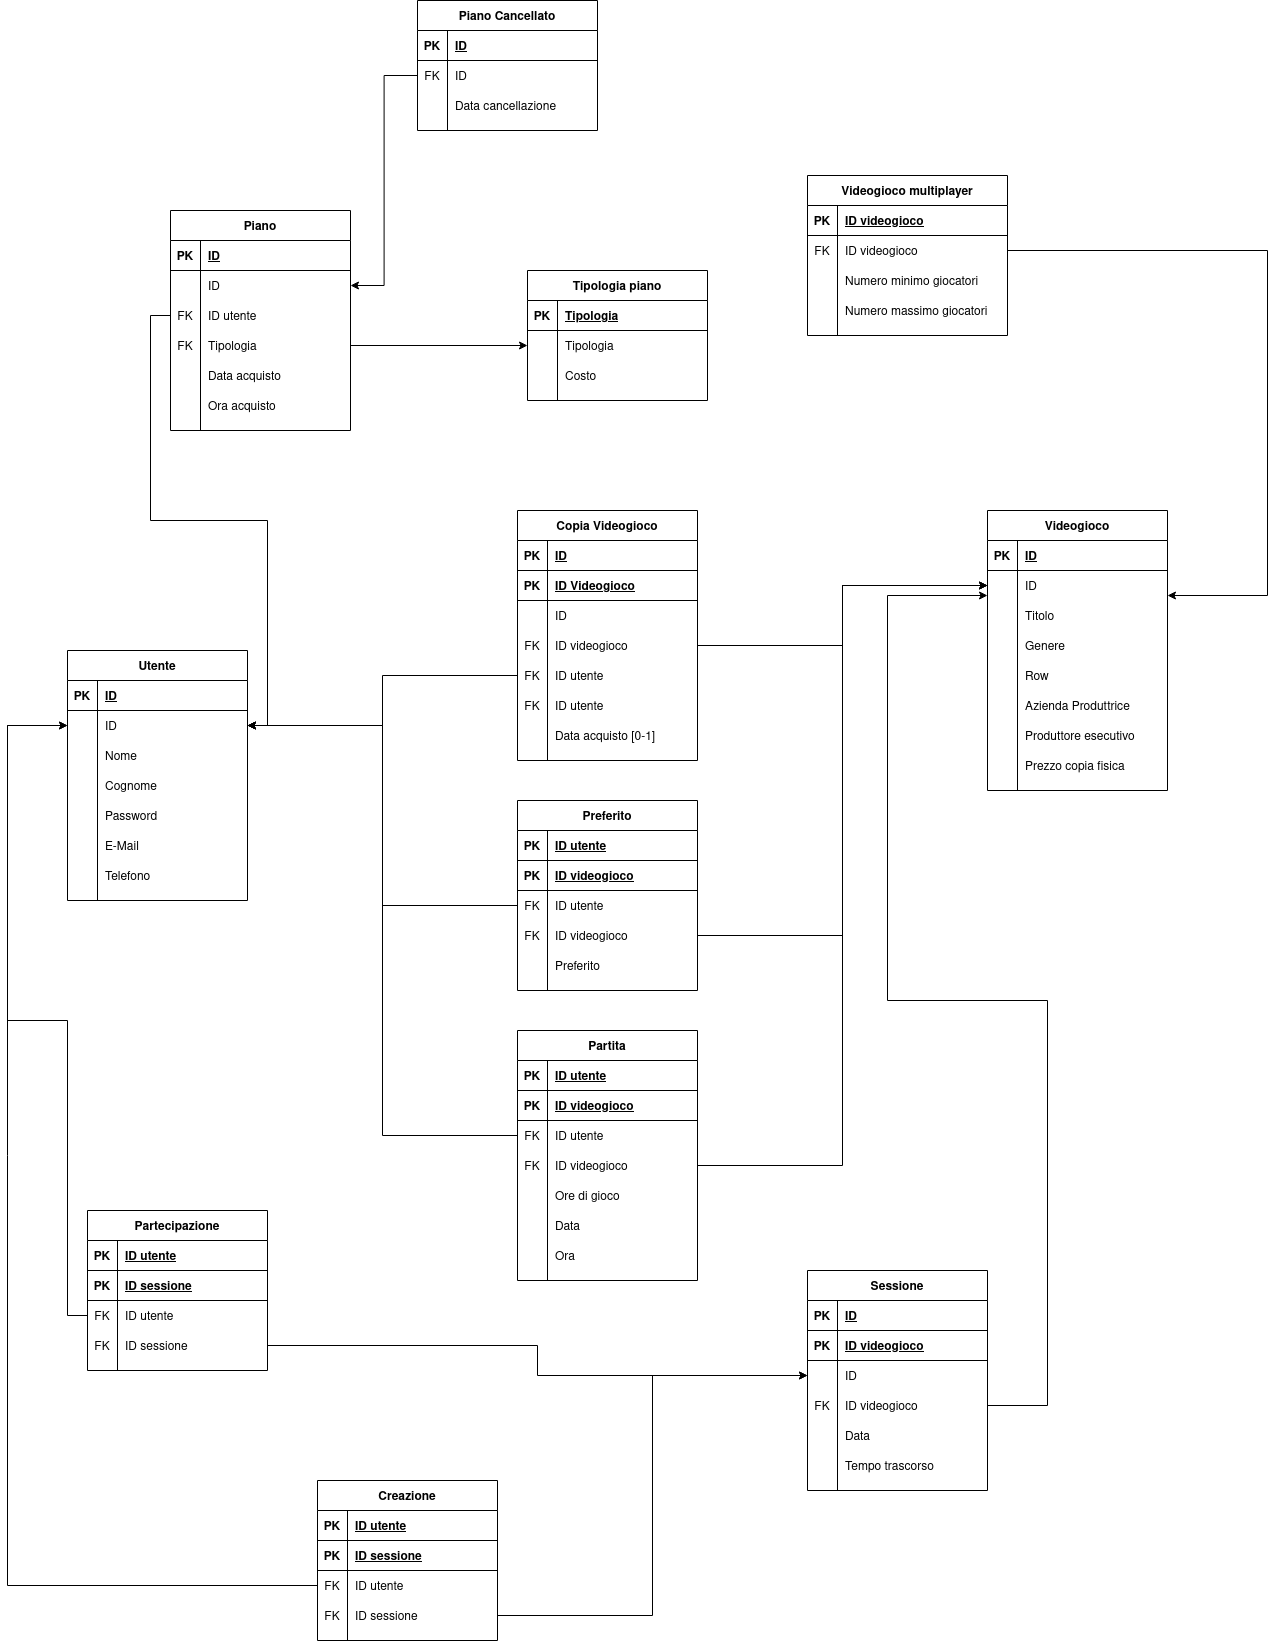
\includegraphics[width=\textwidth]{logical.png}
\caption{Lo schema logico finale.}
\label{img:schema_logico_finale}
\end{figure}

\newpage

\sect{Costruzione delle tabelle in linguaggio SQL}

\begin{lstlisting}

create table Utente (
    id              int                 primary key auto_increment,
    nome            varchar(255)        not null,
    cognome         varchar(255)        not null,
    password        varchar(255)        not null,
    email           varchar(255)        not null,
    telefono        int
);

create table Videogioco (
    id              int                 primary key auto_increment,
    titolo          varchar(255)        not null,
    genere          varchar(255),
    anno            year,
    azienda         varchar(255),
    produttore      varchar(255),
    prezzo          int
);

create table CopiaVideogioco (
    id              int                 primary key auto_increment,
    id_vg           int                 not null references Videogioco(id)
);

create table Acquisto (
    id_copia        int                 not null references CopiaVideogioco(id),
    id_usr          int                 not null references Utente(id),
    data_acquisto   date,
    ora_acquisto    time,
    unique (id_copia, id_usr)
);

create table Partita (
    id_usr          int                 not null references Utente(id),
    id_vg           int                 not null references Videogioco(id),
    data            date                not null,
    ora             time                not null,
    ore_gioco       int,
    unique (id_usr, id_vg, data, ora)
);

create table Preferenza (
    id_usr          int                 not null references Utente(id),
    id_vg           int                 not null references Videogioco(id),
    unique (id_usr, id_vg)
);

create table VideogiocoMultiplayer (
    id_vg           int                 primary key references Videogioco(id),
    min_giocatori   int                 default 1,
    max_giocatori   int
);

create table TipologiaPiano (
    tipologia       enum('Gratuito',
                         'Mensile',
                         'Annuale')     primary key,
    costo           int                 not null
);

create table Piano (
    id              int                 primary key auto_increment,
    id_usr          int                 not null references Utente(id),
    tipologia       enum('Gratuito',
                         'Mensile',
                         'Annuale')     not null references TipologiaPiano(tipologia),
    data_acquisto   date                not null,
    ora_acquisto    time                not null,
    data_fine       date                not null,
    ora_fine        time                not null
);

create table PianoCancellato (
    id              int                 primary key references Piano(id),
    data_canc       date                not null,
    ora_canc        time                not null
);

create table Sessione (
    id              int                 primary key auto_increment,
    id_vg           int                 not null references VideogiocoMultiplayer(id_vg),
    id_creatore     int                 not null references Utente(id),
    data            date,
    ora             time,
    tempo_trascorso int
);

create table Partecipazione (
    id_usr          int                 not null references Utente(id),
    id_session      int                 not null references Sessione(id),
    unique(id_usr, id_session)
);

\end{lstlisting}

\sect{Traduzione delle operazioni in query SQL}

\subsection*{1. Login di un utente}

    \begin{lstlisting}
    select *
    from Utente u
    where u.nome = nome_utente
    and u.cognome = cognome_utente
    and u.password = password_utente;
    \end{lstlisting}

\subsection*{2. Registrare la sottoscrizione di un piano}

Per verificare se l'utente ha già un piano, la seguente query non deve restituire nessun record. Il risultato di questa query è l'ID del piano corrente dell'utente, che dovrà inoltre essere l'unico valido se l'utente ha già sottoscritto un piano (la certezza di ciò si ottiene per come si gestisce l'aggiunta e cancellazione dei piani).

    \begin{lstlisting}
    select id as id_piano
    from Piano p
    where p.id_usr = id_utente
    and datediff(now(), p.data_fine) < 0
    and p.id not in (
        select pc.id
        from PianoCancellato pc
    );
    \end{lstlisting}

Se tale condizione risulta soddisfatta (nessun ID trovato), allora si procede con l'inserimento di un nuovo piano.

	\begin{lstlisting}
    insert into Piano(id_usr, tipologia, data_acquisto, ora_acquisto, data_fine, ora_fine) values(id_utente, ?, now(), now(), ?, now());
    \end{lstlisting}

\subsection*{3. Registrare la cancellazione di un piano}

L'operazione riutilizza la query di condizione descritta per l'operazione sopra: in questo caso, la query deve restituire l'ID del piano (invece di nulla), che poi sarà memorizzato per essere utilizzato nell'inserimento.
Dopo aver effettivamente trovato e memorizzato l'ID, si può procedere nell'inserimento.

    \begin{lstlisting}
    insert into PianoCancellato(id, data_canc, ora_canc) values(id_piano, now(), now());
    \end{lstlisting}

\subsection*{4. Cercare un gioco per titolo/genere/azienda e usando un filtro}

Si presuppone che la scelta della colonna su cui avvenga il filtraggio venga fatto a lato software.

    \begin{lstlisting}
    select id, titolo as Titolo, genere as Genere, azienda as Azienda
    from Videogioco vg
    where vg.? like '%%?%%';
    \end{lstlisting}

\subsection*{5. Visualizzare i giochi più giocati e quelli più preferiti}

    \begin{lstlisting}
    select id, vg.titolo as Titolo, vg.genere as Genere, vg.azienda as Azienda, count(id_usr) as Preferenza
    from Preferenza p, Videogioco vg
    where p.id_vg = vg.id
    group by id_vg
    order by Preferenza desc
    limit 5;
    \end{lstlisting}

	\begin{lstlisting}
    select id, vg.titolo as Titolo, vg.genere as Genere, vg.azienda as Azienda, count(p.ore_gioco) as Ore
    from Partita p, Videogioco vg
    where vg.id = p.id_vg
    group by id_vg
    order by Ore desc
    limit 5;
    \end{lstlisting}

\subsection*{6. Registrare l'acquisto di una copia di un videogioco}

La seguente query trova il numero di copie disponibili per il videogioco scelto: per controllare se si può effettuare un acquisto, basta controllare che num\_disponibili != 0. La query inoltre sceglie, in caso di copie disponibili, l'ID di una copia da comprare: questa viene scelta in base all'ID più basso tra le copie disponibili. La query restituisce anche il prezzo del videogioco, usabile per un eventuale sistema di pagamento dentro l'applicazione.

    \begin{lstlisting}
    select min(cv.id) as id_da_comprare, count(*) as numero_copie, vg.prezzo as prezzo
    from CopiaVideogioco cv, Videogioco vg
    where vg.id = id_videogioco
    and cv.id_vg = vg.id
    and cv.id not in (
    		select id_copia
    		from Acquisto
    	);
    \end{lstlisting}

Dopo essersi accertato della condizione e aver estratto l'ID della copia da compare, si può procedere con l'acquisto.

    \begin{lstlisting}    
    insert into Acquisto(id_copia, id_usr, data_acquisto, ora_acquisto) values(id_da_comprare, id_utente, now(), now());
    \end{lstlisting}

\subsection*{7. Cercare un utente usando un filtro}

    \begin{lstlisting}
    select id, nome as Nome, cognome as Cognome
    from Utente u
    where u.nome like '%%nome_utente%%'
    or u.cognome like '%%cognome_utente%%'
    \end{lstlisting}

\subsection*{8. Visualizzare il numero di ore di gioco giornaliero e totale di un utente}

La seguente query restituisce la media delle ore per ogni giorno.

    \begin{lstlisting}
    select avg(p.ore_gioco) as 'Ore giornaliere'
    from Partita p
    where p.id_usr = id_utente
    group by p.data;
    \end{lstlisting}

La seguente query invece restituisce le ore totali.

    \begin{lstlisting}
    select count(ore_gioco) as 'Ore totali'
    from Partita
    where id_usr = id_utente
    \end{lstlisting}

\subsection*{9. Visualizzare i giochi preferiti di un utente}

    \begin{lstlisting}
    select vg.id, vg.titolo as Titolo
    from Videogioco vg, Preferenza p
    where vg.id = p.id_vg
    and p.id_usr = id_utente;
    \end{lstlisting}

\subsection*{10. Aggiungere un gioco tra i preferiti}

Non dovrebbe essere necessario dover fare un controllo, dato che per costruzione del database, la tabella Preferenza non ammette coppie utente-videogioco uguali.

    %\begin{lstlisting}
    %select *
    %from Preferenza p
    %where p.id_usr = id_utente
    %and p.id_vg = id_videogioco
	%\end{lstlisting}

    \begin{lstlisting}
    insert into Preferenza(id_usr, id_vg) values(id_utente, id_videogioco);
    \end{lstlisting}

\subsection*{11. Registrare la creazione di una sessione di gioco}

La seguente query esegue il controllo descritto quando è stata descritta l'operazione nella sezione delle tabelle degli accessi: controlla se il videogioco è multiplayer e se supporta il numero di giocatori che vogliono partecipare.

    \begin{lstlisting}
    select *
    from VideogiocoMultiplayer
    where id_vg = id_videogioco
    and min_giocatori <= num_giocatori
    and max_giocatori >= num_giocatori;
    \end{lstlisting}

Dopo aver fatto il controllo, si può procedere con l'inserimento: dato che per l'inserimento in Partecipazione ci serve sapere l'ID della sessione, bisogna prima inserire dentro Sessione, poi dentro Partecipazione.

    \begin{lstlisting}
    insert into Sessione(id_vg, id_creatore, data, ora, tempo_trascorso) values(id_videogioco, id_utente, now(), now(), ?);
    \end{lstlisting}
    
    \begin{lstlisting}
    insert into Partecipazione(id_usr, id_session) values(id_utente, last_insert_id());
    \end{lstlisting}
    
\subsection*{12. Visualizzare quante sessioni un utente ha creato o ha partecipato per un videogioco}

    \begin{lstlisting}
    select tb2.vg2, tb2.Titolo, ifnull(tb1.creat, 0) as Creazioni, tb2.part as Partecipazioni from (
        select vg.id as vg1, vg.titolo, count(s.id) as creat
        from Videogioco vg, Sessione s
        where vg.id = s.id_vg
        and s.id_creatore = %1
        group by vg.id
    ) as tb1 right join (
        select vg.id as vg2, vg.titolo as titolo, count(s.id) as part
        from Partecipazione p, Sessione s, Videogioco vg
        where p.id_session = s.id
        and s.id_vg = vg.id
        and p.id_usr = %1
        group by vg.id
    ) as tb2 on vg1 = vg2
    \end{lstlisting}

\subsection*{13. Visualizzare il profitto mensile del servizio}

La query restituisce il profitto per un singolo mese-anno scelto dall'utente.

    \begin{lstlisting}
    select sum(profits) from (
        select sum(vg.prezzo) as profits
        from CopiaVideogioco cv, Acquisto a, Videogioco vg
        where a.id_copia = cv.id and vg.id = cv.id_vg
        and extract(year_month from a.data_acquisto) = 'anno_mese'

        union

        select sum(costo)
        from Piano p, TipologiaPiano tp
        where p.tipologia = tp.tipologia
        and extract(year_month from p.data_acquisto) = 'anno_mese'
    ) as tb;
    \end{lstlisting}

\chap{Progettazione dell'applicazione}

\sect{Descrizione dell'architettura dell'applicazione}

L'applicazione da interfaccia al database è stata realizzata in linguaggio C++: l'applicazione è una semplice Qt App, che sfrutta le librerie di Qt per collegarsi ad un database in locale. Il DBMS usato è MariaDB, un DBMS compatibile con MySQL.

L'architettura segue il Model-View-View-Model, un pattern molto seguito anche dalle librerie usate. Il model è composto da una serie di funzioni, che permettono di connettersi al database e di effettuare le operazioni basilari descritte in questa relazione. La view invece è rappresentata dalle classi che rappresentano la finestra e i widget dell'applicazione, che sfruttano il pattern Observer: all'arrivo di un evento, queste internamente chiamano una delle funzioni del model e gestiscono i dati in output dell'operazione.

\begin{figure}[H]
\centering{}
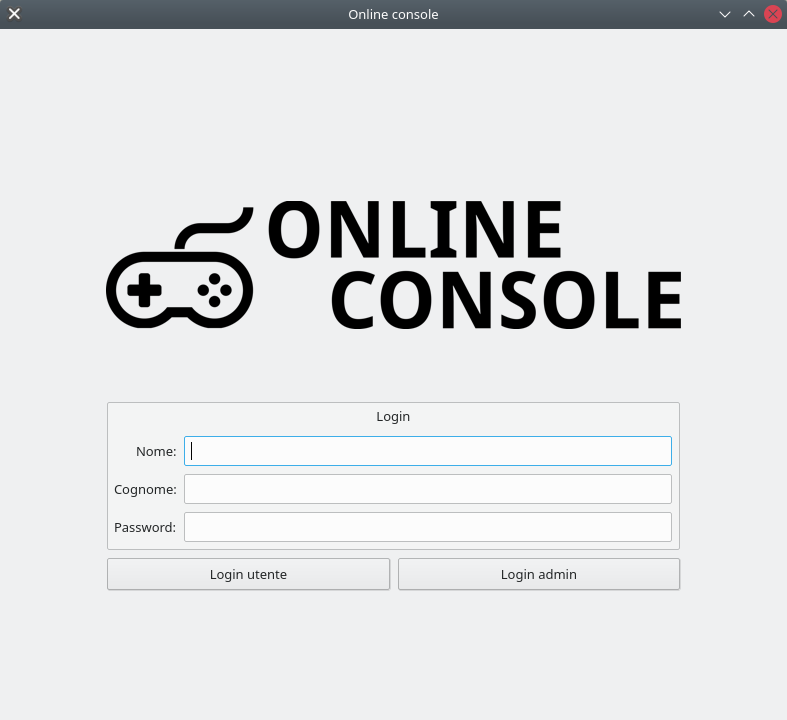
\includegraphics[width=12cm]{screen_login.png}
\caption{La schermata di login.}
\label{img:screen_login}
\end{figure}

L'applicazione si presenta con una finestra di login: qui è possibile fare il login sia come utente, sia come admin. La validazione per gli utenti viene fatta tramite una query al database. Per semplicità, non è stato implementato alcun sistema di criptazione delle password: queste sono memorizzate in chiaro nel database.

\begin{figure}[H]
\centering{}
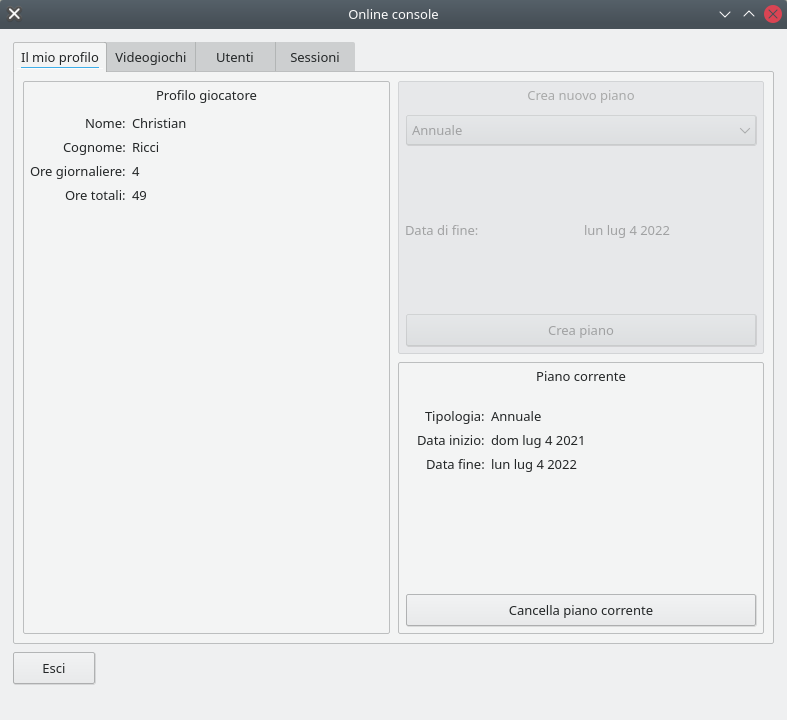
\includegraphics[width=12cm]{screen_profile.png}
\caption{Il profilo dell'utente.}
\label{img:screen_login}
\end{figure}

Dopo che un utente ha fatto il login, viene presentata una schermata che mostra il profilo dell'utente e il suo piano in corso. Se non l'utente non ha ancora sottoscritto un piano, lo può fare tramite un form: basta scegliere la tipologia di piano e cliccare sul pulsante "Crea". Questo pulsante andrà subito ad inserire un nuovo piano nel database e renderà disponibile la visualizzazione delle altre schermate. Cliccando sul pulsante "Cancella", il piano in corso verrà subito cancellato e all'utente sarà privata la possibilità di visualizzare le altre schermate.

\begin{figure}[H]
\centering{}
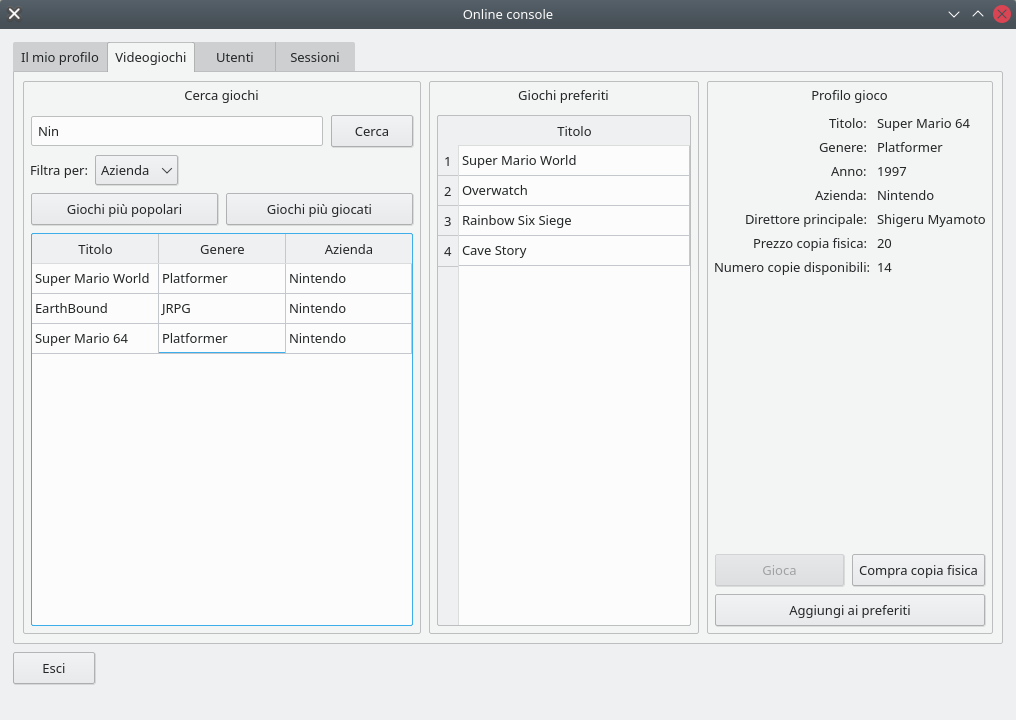
\includegraphics[width=12cm]{screen_games.png}
\caption{La schermata relativa ai videogiochi.}
\label{img:screen_login}
\end{figure}

Nella schermata videogiochi, l'utente può cercare videogiochi e visualizzare i suoi giochi preferiti. La ricerca avviene digitando del testo nella casella e filtrando per titolo, genere o azienda sviluppatrice. Si può anche ignorare la ricerca e visualizzare i giochi più giocati o i giochi più preferiti. Cliccando sul nome di un videogioco, sia nella tabella dei risultati di ricerca, sia nella tabella dei preferiti, viene mostrato un profilo sul videogioco, che contiene tutte le informazioni di base. Tramite i bottoni sul profilo, l'utente può giocare al videogioco e può metterlo tra i suoi preferiti o comprarne una copia fisica. Il bottone "gioca" è stato disabilitato, dato che in questa applicazione non c'è nessun sistema di gioco; inoltre, per semplicità non è stato inserito nessun sistema di pagamento: cliccando sul pulsante "compra", si procede subito all'acquisto.

\begin{figure}[H]
\centering{}
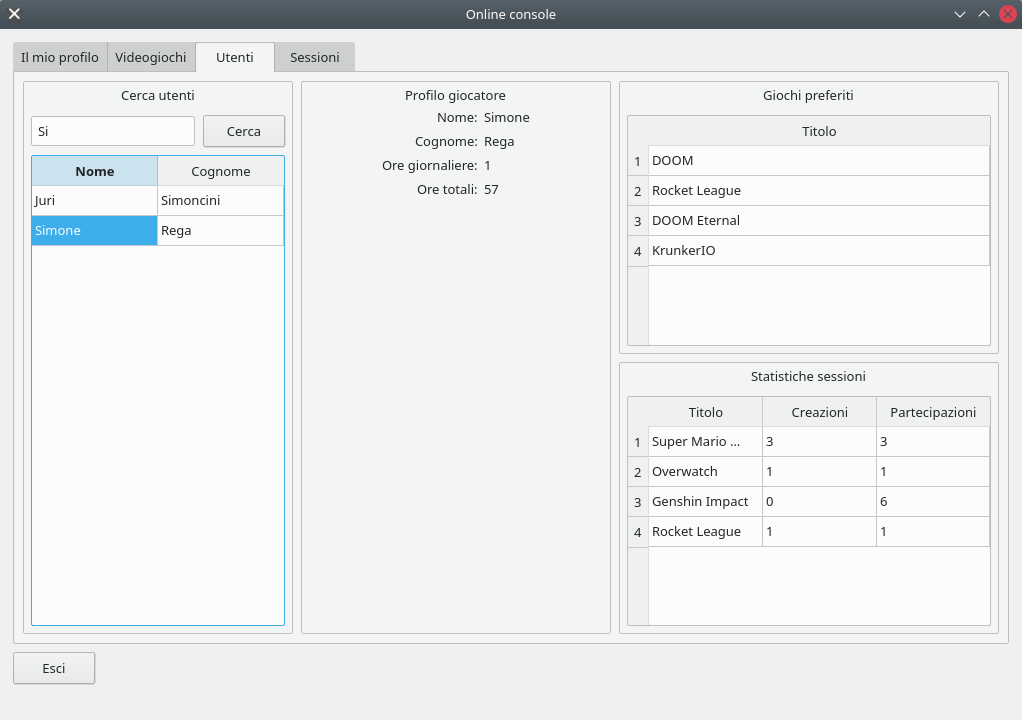
\includegraphics[width=12cm]{screen_users.png}
\caption{Ricerca e visualizzazione del profilo degli altri utenti.}
\label{img:screen_login}
\end{figure}

Nella schermata relativa agli utenti, si possono cercare gli utenti e, cliccando sul nome di un utente, si può visualizzare il relativo profilo. Oltre alle informazioni basilari, vengono anche mostrate due tabelle contenenti i giochi preferiti dell'utente che si sta visualizzando e anche il numero di sessioni in cui ha partecipato/creato, organizzate per videogioco.

\begin{figure}[H]
\centering{}
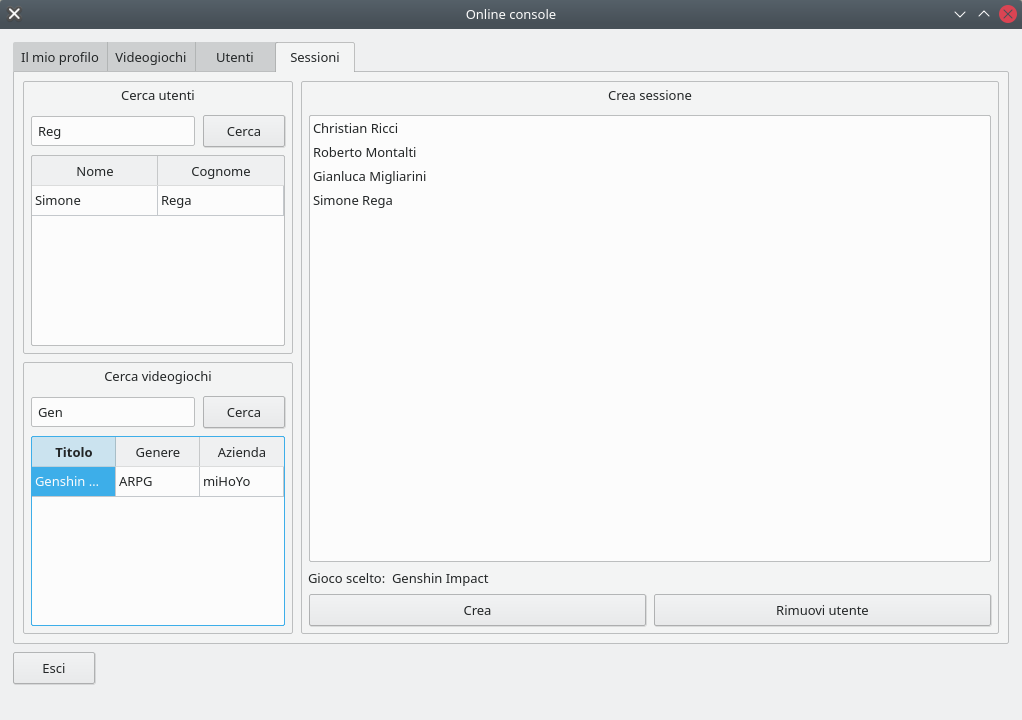
\includegraphics[width=12cm]{screen_sessions.png}
\caption{La schermata relativa alle sessioni di gioco.}
\label{img:screen_login}
\end{figure}

L'ultima schermata è relativa alle sessioni: è cui che si possono iniziare sessioni di gioco con altri utenti. Gli utenti si possono inserire cercando e cliccando sul nome di un utente; la scelta del videogioco viene in maniera analoga alla selezione degli utenti, e il nome del videogioco compare sotto la lista degli utenti selezionati. Il pulsante "Rimuovi utente" rimuove un utente dalla lista e non fa alcuna operazione; il pulsante "Crea" crea una nuova sessione di gioco con gli utenti e il gioco selezionato. Ancora una volta, per semplicità, non è stato inserito nessun sistema di gioco, e l'applicazione andrà subito ad inserire una nuova sessione nel database, con il tempo trascorso scelto in maniera casuale.

\begin{figure}[H]
\centering{}
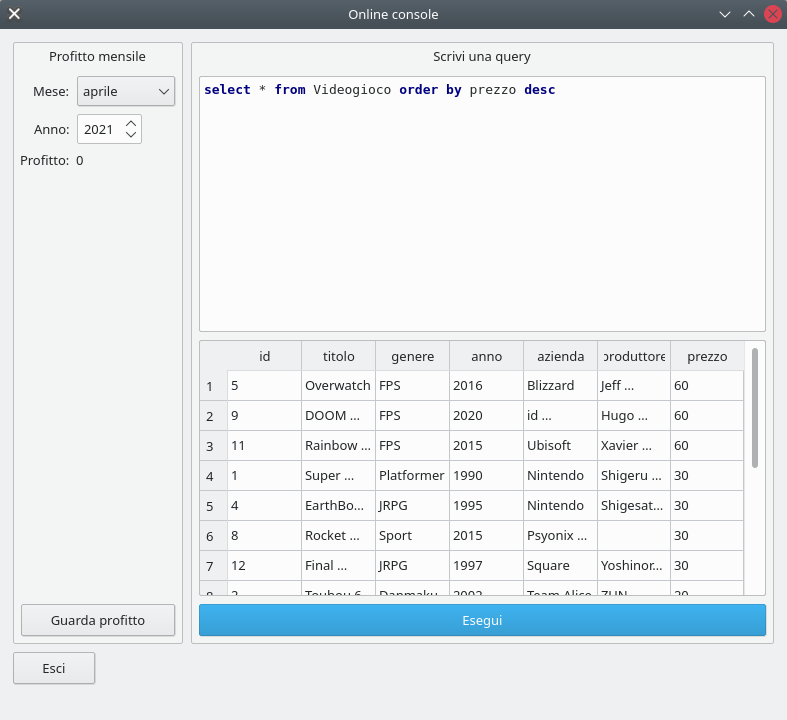
\includegraphics[width=12cm]{screen_admin.png}
\caption{La schermata dell'amministratore.}
\label{img:screen_login}
\end{figure}

Oltre alla schermate per l'utente esiste anche una schermata per il Database Administrator: questa è accessibile tramite il pulsante relativo nella schermata di login. La schermata di amministratore contiene principalmente un form per sapere il profitto del servizio in un certo mese, e un editor di query per fare delle query SQL generiche al database. Cliccando sul pulsante "Guarda profitto", dopo aver scelto mese e anno, comparira il valore del profitto in quel mese, mentre cliccando sul pulsante "Esegui", verrà eseguita la query scritta nell'editor.

\end{document}
